% !TEX program = pdflatex
% WordleGym supplementary writeup.

\documentclass[11pt]{article}

\usepackage[margin=0.9in]{geometry}
\usepackage{amsmath, amssymb, amsthm}
\usepackage{booktabs}
\usepackage{array}
\usepackage{microtype}
\usepackage{siunitx}
\usepackage[round,authoryear]{natbib}
\usepackage{pgfplots}
\pgfplotsset{compat=1.18}
\usepgfplotslibrary{colorbrewer}
\usepackage{hyperref}
\usepackage{xcolor}
\usepackage{xstring}

\definecolor{stratEntropy}{HTML}{2563EB}
\definecolor{stratCandElim}{HTML}{8B5CF6}
\definecolor{stratMinimax}{HTML}{EF4444}
\definecolor{stratPosteriorHybrid}{HTML}{10B981}
\definecolor{stratPosteriorExp}{HTML}{0891B2}
\definecolor{stratEvilSP}{HTML}{BE185D}
\definecolor{stratRobust}{HTML}{475569}
\definecolor{stratLetterFreq}{HTML}{F59E0B}
\definecolor{stratRandom}{HTML}{94A3B8}
\definecolor{stratEvilDP}{HTML}{16A34A}

% ── Wordle tile graphics (reusable across games) ───────────────────
% Palette matches the canonical Wordle UI. Use \wG, \wY, \wB, \wE
% for a single tile, or \wrow{LETTERS}{PATTERN} for a 5-tile row.
%   PATTERN is a five-character string drawn from {G, Y, B, E}:
%     G = green  (correct letter, correct position)
%     Y = yellow (correct letter, wrong position)
%     B = gray   (letter absent)        [B for "black" / "blank"]
%     E = empty  (turn not yet played)
\definecolor{wordleGreen}{HTML}{6AAA64}
\definecolor{wordleYellow}{HTML}{C9B458}
\definecolor{wordleGray}{HTML}{787C7E}
\definecolor{wordleEmpty}{HTML}{D3D6DA}

\newlength{\wtilesize}\setlength{\wtilesize}{5.4mm}
\newcommand{\wtilefont}{\bfseries\sffamily}

% Single tile. Args: letter, fill colour, text colour.
\newcommand{\wtileC}[3]{%
  \tikz[baseline=(t.base)]{
    \node[fill=#2, text=#3, font=\wtilefont,
          minimum width=\wtilesize, minimum height=\wtilesize,
          inner sep=0pt, outer sep=0.4pt] (t) {\MakeUppercase{#1}};%
  }%
}
\newcommand{\wG}[1]{\wtileC{#1}{wordleGreen}{white}}
\newcommand{\wY}[1]{\wtileC{#1}{wordleYellow}{white}}
\newcommand{\wB}[1]{\wtileC{#1}{wordleGray}{white}}
\newcommand{\wE}[1]{\wtileC{#1}{wordleEmpty}{black!55}}

% \wrow{LETTERS}{PATTERN} - draw a five-tile row.
%   \wrow{CRANE}{BYYBY} renders C-R-A-N-E with feedback gray-yellow-yellow-gray-yellow.
\newcommand{\wrow}[2]{%
  \StrChar{#1}{1}[\wxA]\StrChar{#2}{1}[\wyA]%
  \StrChar{#1}{2}[\wxB]\StrChar{#2}{2}[\wyB]%
  \StrChar{#1}{3}[\wxC]\StrChar{#2}{3}[\wyC]%
  \StrChar{#1}{4}[\wxD]\StrChar{#2}{4}[\wyD]%
  \StrChar{#1}{5}[\wxE]\StrChar{#2}{5}[\wyE]%
  \mbox{%
    \csname w\wyA\endcsname{\wxA}%
    \csname w\wyB\endcsname{\wxB}%
    \csname w\wyC\endcsname{\wxC}%
    \csname w\wyD\endcsname{\wxD}%
    \csname w\wyE\endcsname{\wxE}%
  }%
}

% ── Per-turn decision-table row ───────────────────────────────────
% Markers used inside the top-5 mini-tables:
%   \dchosen  = chosen by the strategy at this turn (bold + filled star)
%   \dcand    = currently in the candidate pool (open diamond)
%   \dnone    = neither (blank slot, keeps column alignment)
\newcommand{\dchosen}{\hbox to 1.1em{\hfil$\bigstar$\hfil}}
\newcommand{\dcand}{\hbox to 1.1em{\hfil$\diamond$\hfil}}
\newcommand{\dnone}{\hbox to 1.1em{\hfil}}

% Per-strategy decision panel.
%   \decpanel{strategy-id}{metric line}{tabular-body}
% The tabular body has columns:  turn-info | tile-row | mini top-5 table.
\newcommand{\decpanel}[3]{%
  \par\addvspace{6pt}%
  \noindent\textcolor{black!18}{\rule{\linewidth}{0.6pt}}\par
  \smallskip
  \noindent
  {\sffamily\bfseries\normalsize\texttt{#1}}%
    \quad{\sffamily\footnotesize\color{black!55}#2}\par
  \smallskip
  \begin{center}\footnotesize
  \renewcommand{\arraystretch}{1.15}%
  \begin{tabular}{@{}l c l@{}}
  \toprule
  \multicolumn{1}{c}{\textbf{Turn}} &
    \multicolumn{1}{c}{\textbf{Play}} &
    \multicolumn{1}{c}{\textbf{Top 5 by metric}}\\
  \midrule
  #3
  \bottomrule
  \end{tabular}
  \end{center}
  \par\addvspace{6pt}%
}

% ── Per-strategy trajectory panel ─────────────────────────────────
% \trajpanel{name}{tier-label}{turns}{tile-rows}{analysis}
% Renders a labeled, divider-separated panel with tile rows on the
% left and analysis prose on the right. Use \\[2pt] between rows
% inside the tile-rows arg so adjacent rows don't touch.
\newlength{\trajpanelskip}\setlength{\trajpanelskip}{6pt}
\newcommand{\trajpanel}[5]{%
  \par\addvspace{\trajpanelskip}%
  \noindent\textcolor{black!18}{\rule{\linewidth}{0.6pt}}\par
  \smallskip
  \noindent
  {\sffamily\bfseries\normalsize\texttt{#1}}%
    \quad{\sffamily\footnotesize\color{black!55}#2 \,$\cdot$\, #3 turns}\par
  \smallskip
  \noindent
  \begin{minipage}[t]{0.34\linewidth}%
    \centering #4%
  \end{minipage}%
  \hfill
  \begin{minipage}[t]{0.62\linewidth}%
    \footnotesize\setlength{\parskip}{3pt}#5%
  \end{minipage}%
  \par\addvspace{\trajpanelskip}%
}

\hypersetup{
  colorlinks=true,
  linkcolor=black,
  urlcolor=blue!55!black,
  citecolor=black
}

\newcommand{\fb}{\mathrm{fb}}
\newcommand{\evilT}{T}

\setlength{\parskip}{4pt}
\setlength{\parindent}{0pt}

\title{\textbf{WordleGym:}\\[2pt]\large Benchmarking Wordle Strategies under Standard, Adversarial, and Hidden-Mode Play}
\author{Michael Wang\\
\small Math 242 \textbullet{} Duke University \textbullet{} Spring 2026\\
\small Code: \href{https://github.com/Michael-OvO/WordleGym}{\texttt{github.com/Michael-OvO/WordleGym}}
  \textbullet{}
  Live demo: \href{https://wordlegym.vercel.app/}{\texttt{wordlegym.vercel.app}}}
\date{}

\begin{document}
\maketitle

%====================================================================
\section*{Problem Statement}
%====================================================================

Wordle is a word game in which the player has six guesses to identify a
hidden five-letter word. After each guess, every letter is marked
green (correct letter in the correct position), yellow (correct letter
in the wrong position), or gray (not in the word). From this simple
feedback rule emerges a rich decision problem: with $\num{2315}$
possible answers, which guess at each turn makes the best use of the
remaining information?

To compare strategies rigorously, I built \emph{WordleGym}, a Python
benchmark that plays the game automatically under different policies
and records their performance. I studied three variants of the game in
order to make the analysis more interesting:

\textbf{Standard} is the ordinary game: the answer is fixed at the
start, and feedback is truthful.

\textbf{Evil} is an adversarial version. The game does not commit to
a hidden answer in advance; instead, after each guess it returns the
feedback pattern that preserves the largest number of still-valid
answers. The adversary is cheating, but in a consistent and
deterministic way.

\textbf{Unknown} combines the two. At the start of each game the game
is secretly either Standard or Evil with equal probability, and the
player must infer which from feedback alone.

The central question of the project is how simple, one-step strategies
compare to one another, and how close they come to the best possible
play.

%====================================================================
\section*{Setting Up the Math}
%====================================================================

Some notation is needed before introducing the strategies. At any
point in a game, let $C$ denote the set of words still consistent with
the feedback observed so far. A guess $g$ partitions $C$ into
\emph{buckets}: all words in $C$ that would produce the same feedback
pattern against $g$ fall into the same bucket. Write $B_r$ for the
bucket corresponding to feedback pattern $r$, and $|B_r|$ for the
number of words in it.

Intuitively, a good guess splits $C$ into many small buckets. If one
bucket is large, the guess barely narrows the search; if every bucket
contains only one or two words, the guess is highly informative. This
notion of ``how evenly does a guess split the candidates'' is the
common thread linking all of the strategies I tested.

To make the bucket idea concrete, fix the guess $g = \texttt{CRANE}$
and consider two candidate answers. Against \texttt{AFTER}, the letters
score as gray--yellow--yellow--gray--yellow (C absent; R and A both
present but in the wrong positions; N absent; E present but at the
wrong position). Against \texttt{AMBER}, the letters score identically:
gray--yellow--yellow--gray--yellow. The two answers produce the
\emph{same} five-tile feedback pattern against \texttt{CRANE}, so they
fall in the same bucket $B_{\mathrm{BYYBY}}$ together with 48 other
candidates:
\begin{center}
\begin{tabular}{c c c}
\small answer \texttt{AFTER} & & \small answer \texttt{AMBER}\\[2pt]
\wrow{CRANE}{BYYBY} & \quad$=$\quad & \wrow{CRANE}{BYYBY}\\
\end{tabular}
\end{center}
The important point is that the bucket structure is a property of the
guess alone: the player does not need to know the true answer to
compute it. For every candidate word $w \in C$, the player simulates
``what feedback would the game produce if $w$ were the answer?'' and
tallies the resulting patterns. The player then chooses a guess based
on the shape of that tally --- its entropy, its largest bucket, and so
on --- entirely without reference to the true hidden word.

For each of the three modes, the optimal policy can be written as a
recursion. These recurrences define what a perfect player would do;
every strategy in the benchmark is an approximation to one of them.

In Standard mode, the minimum expected number of remaining guesses from
a candidate set $C$ satisfies
\begin{equation}
  V(C) \;=\; \min_{g}\;\Bigl[\,1 + \!\!\sum_{r \ne \gamma,\,B_r \ne \emptyset}\!
               \tfrac{|B_r|}{|C|}\,V(B_r)\Bigr],
  \qquad V(\{w\}) = 1.
  \label{eq:VC}
\end{equation}
Here $\gamma$ denotes the all-green feedback pattern, which terminates
the game immediately and so contributes no future cost.

\textit{In plain language.} Read the recurrence left to right. ``$V(C)$
is the smallest expected number of guesses needed when the answer is
somewhere in $C$.'' The $\min_g$ says: try every legal guess and keep
the best one. Inside the brackets, the ``$1$'' counts the current guess
itself. The sum is the work that remains \emph{after} the guess: with
probability $|B_r|/|C|$ the feedback comes back as pattern $r$, and
once that happens the player is in exactly the same problem all over
again, only on the smaller candidate set $B_r$. So the bracketed
expression is ``$1$ for this guess, plus the average future cost,
averaged over all the ways the game could turn out.'' Two things make
this ``optimal'': it averages over uncertainty rather than reacting to
worst case, and it is recursive --- the cost of a guess depends on the
costs of the subgames it creates, all the way down to single-word
subsets $V(\{w\}) = 1$ where the answer is known.

In Evil mode, the adversary always returns the largest bucket, so the
player wants to minimize the size of the bucket returned. Letting
$\evilT(C, g)$ denote that adversarial successor bucket,
\begin{equation}
  D(C) \;=\; \min_{g}\;\bigl[\,1 + D(\evilT(C, g))\,\bigr].
  \label{eq:DC}
\end{equation}

In Unknown mode, the player maintains a posterior probability $q$ that
the current game is Standard, updated by Bayes' rule after each
feedback. The optimal policy is a weighted combination of the Standard
and Evil recurrences:
\begin{equation}
  V_U(C) \;=\; \min_{g}\Bigl[\,1 + q\cdot(\text{standard term})
                              + (1{-}q)\cdot(\text{evil term})\Bigr].
  \label{eq:VU}
\end{equation}

These recurrences are the exact optima, but solving them directly
requires searching the entire game tree, which is computationally
prohibitive in pure Python. The benchmark question then becomes: how
well can more tractable, one-step strategies approximate these optima?

\textit{Prior work on the exact Standard-mode optimum.} Recurrence
\eqref{eq:VC} has been solved at Wordle scale by
\citet{bertsimas2022wordle}, published in \emph{Operations Research}
in 2025. They formulate the Bellman equation for $V(C)$, reduce it
with a series of symmetry and dominance pruning steps, and then
compile the resulting policy into an Optimal Classification Tree with
Hyperplanes for interpretability. On the canonical $\num{2315}$-word
answer list they report opening guess \texttt{SALET}, an average of
$V(A) = 3.421$ guesses, and a worst case of $W(A) = 5$: the game
never requires a sixth guess under optimal play.
\citet{selby2022wordle} independently reports the same bounds via a
distinct search procedure. Both solvers rely on compiled languages
and tight data structures, so my pure-Python benchmark does not
attempt to reproduce the Standard-mode DP; instead, every Standard
result below is compared against their published numbers. The
companion notes \texttt{docs/dp-methods.md} and
\texttt{docs/findings.md} in the repository record the full
derivations and a headline summary.

%====================================================================
\section*{Strategies Tested}
%====================================================================

I focus on six strategies, each chosen to occupy a distinct point in
the design space so the comparison stays apples-to-apples without
becoming a catalogue.

\textbf{Baselines.} Two unsophisticated policies set a floor.
\texttt{random-valid} chooses uniformly at random among the
still-valid words --- a reproducibility-seeded control with no
reasoning at all. \texttt{letter-frequency} picks the word whose
letters occur most often among the remaining candidates --- a
``human-style'' heuristic that scores guesses on letter statistics
without ever modeling how the feedback pattern partitions the pool.
The gap between these two rows and any reasoning policy is the
quantitative value the reasoning provides; the gap \emph{between}
the two baselines tells you how far letter coverage alone gets you.

\textbf{One-step heuristics.} Two policies look one turn ahead and
pick the guess that best satisfies a specific local objective:

\begin{itemize}
\item \texttt{expected-entropy} selects the guess with the largest
Shannon \emph{information gain} \citep{shannon1948,sanderson2022wordle},
which corresponds to the most balanced distribution of feedback
buckets.
\item \texttt{minimax} is conservative: it selects the guess whose
\emph{largest} bucket is smallest, guarding against the worst-case
feedback \citep{selby2022wordle}.
\end{itemize}

These two illustrate a core tension: entropy is risk-neutral
(averages over feedback patterns), minimax is risk-averse (plans
against the worst feedback). Both reason only one turn ahead, and
both are intuitively close to optimal.

\textbf{Mode-aware (Unknown).} \texttt{posterior-expectimax} is the
one-ply Bayes-optimal blend for Unknown mode, designed by reading
recurrence~(\ref{eq:VU}) and replacing each branch with its one-ply
proxy. It maintains a posterior $q$ that the current game is Standard
and picks the guess that minimizes
\[
  q\sum_r \tfrac{|B_r|^2}{|C|} \;+\; (1-q)\,|\evilT(C, g)|.
\]
Both terms count candidates remaining --- the Standard term is the
expected residual under a uniform answer, the Evil term is the
adversary's forced bucket --- so the blend is dimensionally clean.
At $q=1$ the score is exactly the Standard squared-count argmin; at
$q=0$ it is the pure evil-bucket minimizer. This is the engineered
strategy for Unknown mode, and the question I asked when designing
it was whether the posterior weighting actually buys anything over
running entropy mode-blind.

\textbf{Evil DP (exact).} For Evil mode, I was able to solve
recurrence~(\ref{eq:DC}) exactly. Because the evil adversary is
deterministic, the reachable game tree contains only a few thousand
distinct states, which is tractable in pure Python. The
\texttt{evil-dp} strategy performs memoized depth-first search over
this tree and returns the true optimum. Details of the algorithm are
given below.

%====================================================================
\section*{Benchmark Results}
%====================================================================

Every strategy played each of the $\num{2315}$ canonical Wordle answers
in Standard and Unknown mode. Evil mode is different: the adversary is
deterministic, and each benchmark policy (including
\texttt{random-valid}, whose tie-breaking is seeded deterministically
from the game history) produces one fixed playthrough. The entire Evil
column therefore comes from a single game per row: ``Depth'' and
``WC'' are identical by construction, and both mean turns to solve.
\footnote{The \texttt{random-valid} Evil row solves
in 7 turns under its fixed seed. A separate Monte Carlo run with true
randomness would produce a distribution around this value; I kept the
deterministic seed so that Evil results remain reproducible across
benchmark runs.} ``Mean'' and ``WC'' in the Standard and Unknown
columns are a genuine average and maximum over the 2315-answer pool.
The best value in each column is in \textbf{bold}.

\begin{center}\small
\renewcommand{\arraystretch}{1.1}
\begin{tabular}{@{}l S[table-format=1.3] c S[table-format=1.3] c S[table-format=1.3] c@{}}
\toprule
& \multicolumn{2}{c}{Standard} & \multicolumn{2}{c}{Evil} & \multicolumn{2}{c}{Unknown}\\
\cmidrule(lr){2-3}\cmidrule(lr){4-5}\cmidrule(lr){6-7}
Strategy & {Mean} & {WC} & {Depth} & {WC} & {Mean} & {WC}\\
\midrule
expected-entropy       & \bfseries 3.465 & 6 & 5 & 5 & \bfseries 4.232 & 6 \\
posterior-expectimax   & 3.485 & \bfseries 5 & 5 & 5 & 4.248 & \bfseries 5 \\
minimax                & 3.573 & 6 & 5 & 5 & 4.287 & 6 \\
letter-frequency       & 3.587 & 8 & 5 & 5 & 4.294 & 8 \\
random-valid           & 4.124 & 9 & 7 & 7 & 4.996 & 9 \\
\midrule
\textit{evil-dp (optimal)}& \textit{---} & \textit{---} & \bfseries 4 & \bfseries 4 & \textit{---} & \textit{---} \\
\midrule
Published optimum \citep{bertsimas2022wordle,selby2022wordle}
                       & \bfseries 3.421 & \bfseries 5 & \bfseries 4 & \bfseries 4 & \emph{---} & \emph{---} \\
\bottomrule
\end{tabular}
\end{center}

The same data is more striking as a scatter of average against
worst-case guesses in Standard mode (Figure~\ref{fig:scatter}). The
Pareto frontier of policies runs along the lower-left edge, where
small gains in average performance come at the cost of larger worst
cases.

\begin{figure}[h]
\centering
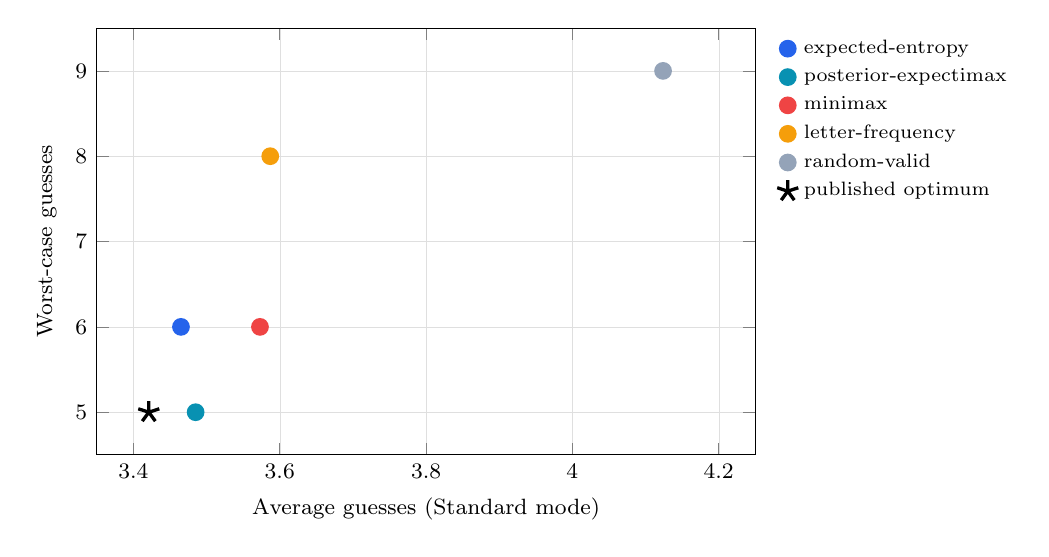
\begin{tikzpicture}
\begin{axis}[
  width=0.82\linewidth, height=7cm,
  xlabel={Average guesses (Standard mode)},
  ylabel={Worst-case guesses},
  xmin=3.35, xmax=4.25,
  ymin=4.5, ymax=9.5,
  ytick={5,6,7,8,9},
  grid=both,
  major grid style={line width=.1pt,draw=gray!25},
  minor grid style={line width=.1pt,draw=gray!10},
  legend style={
    at={(1.02,1)}, anchor=north west,
    font=\scriptsize, cells={anchor=west},
    draw=none, fill=none,
  },
  tick label style={font=\footnotesize},
  label style={font=\footnotesize},
  every axis plot/.append style={mark size=2.8pt, thick},
]
\addplot[only marks, mark=*, color=stratEntropy]          coordinates {(3.465, 6)};
\addplot[only marks, mark=*, color=stratPosteriorExp]     coordinates {(3.485, 5)};
\addplot[only marks, mark=*, color=stratMinimax]          coordinates {(3.573, 6)};
\addplot[only marks, mark=*, color=stratLetterFreq]       coordinates {(3.587, 8)};
\addplot[only marks, mark=*, color=stratRandom]           coordinates {(4.124, 9)};
\addplot[only marks, mark=star, mark size=4pt, color=black, very thick] coordinates {(3.421, 5)};
\legend{
  expected-entropy, posterior-expectimax, minimax, letter-frequency,
  random-valid, published optimum
}
\end{axis}
\end{tikzpicture}
\caption{Average vs.\ worst-case guesses by strategy in Standard mode.
The black star marks the published DP optimum of
\citet{bertsimas2022wordle,selby2022wordle}. Points closer to the
lower-left corner are strictly better.}
\label{fig:scatter}
\end{figure}

Three observations from this table are worth emphasizing.

First, entropy is a surprisingly strong heuristic. The best one-step
policy, \texttt{expected-entropy}, averages $3.465$ guesses in
Standard mode, while the published optimum reported by
\citet{bertsimas2022wordle} is $3.421$ --- a gap of only $0.04$
guesses, or roughly $1.3\%$ above the optimum. A strategy that reasons
only a single turn ahead is within a rounding error of the exact
dynamic-programming optimum.

Second, average and worst-case performance are genuinely different
objectives. \texttt{expected-entropy} has the best Standard-mode
average but permits occasional six-guess games. The mode-aware
\texttt{posterior-expectimax} has a slightly worse average but caps
its worst case at $5$. Minimizing one of these quantities does not,
in general, minimize the other.

Third, the adversary is less powerful than intuition suggests. Every
non-random strategy solves Evil mode in at most $5$ guesses, and the
exact DP solver (\texttt{evil-dp}) solves it in $4$, matching the
known optimum. Notably, $D(A) = 4$ is strictly less than the
Standard-mode worst case of $W(A) = 5$: there exist specific fixed
Wordle answers that are harder than anything the adversary can
construct. The Evil tie-breaking rule, which forces the adversary to
prefer the largest single bucket, removes enough flexibility that a
well-chosen guess sequence can always corner the game.

%====================================================================
\section*{Same Strategies, Two Worlds}
%====================================================================

Aggregate averages hide what is actually happening turn by turn. To
make the differences between strategies concrete, this section freezes
each policy in two settings and watches it play. Standard mode commits
to a hidden answer (\texttt{ABACK}) and returns truthful feedback;
Evil mode commits to nothing and returns the feedback pattern that
preserves the largest set of still-valid answers. The same six
strategies face both worlds, and the same per-turn machinery decides
each guess. The question is which one-step heuristics survive the
transition from a fixed target to an adversarial moving one.

The Standard answer \texttt{ABACK} is chosen deliberately: its
double-A together with the \texttt{B--C--K} consonant cluster falls
outside the usual letter-frequency distribution, so different local
objectives produce visibly different paths. In Evil mode, every
strategy plays only one game --- the adversary's deterministic
play-out from the all-candidates pool --- so the natural comparison
is the single-game record itself.

%--------------------------------------------------------------------
\subsection*{Standard mode \textbullet{} hidden answer \texttt{ABACK}}
%--------------------------------------------------------------------

Solve depth across the six policies ranges from $3$ to $5$, and the
differences are entirely attributable to which one-step quantity each
policy was designed to optimize. Table~\ref{tab:aback-trace-std}
shows every play.

\begin{table}[h]
\centering\footnotesize
\renewcommand{\arraystretch}{1.05}
\begin{tabular}{@{}l l l l l l l@{}}
\toprule
Strategy & Guess 1 & Guess 2 & Guess 3 & Guess 4 & Guess 5 & Turns\\
\midrule
\texttt{minimax}              & arise & clout & \textbf{aback} & ---   & ---   & \textbf{3}\\
\texttt{evil-dp}              & raise & cloak & abuna & \textbf{aback} & ---   & 4\\
\texttt{posterior-expectimax} & roate & slick & abuna & \textbf{aback} & ---   & 4\\
\texttt{expected-entropy}     & soare & clink & aahed & \textbf{aback} & ---   & 4\\
\texttt{random-valid}         & fiery & would & mamma & \textbf{aback} & ---   & 4\\
\texttt{letter-frequency}     & slate & crank & quack & whack & \textbf{aback} & 5\\
\bottomrule
\end{tabular}
\caption{Every strategy's complete Standard-mode game against the
hidden answer \texttt{ABACK}. Solve depth varies from $3$ to $5$
turns even though every policy receives identical feedback rules and
candidate pools. The differences come entirely from the
\emph{local objective} each policy optimizes.}
\label{tab:aback-trace-std}
\end{table}

Six strategies, six distinct trajectories: every policy chooses a
different opener. \texttt{minimax} is the outlier on the upside,
solving in three because its turn-2 probe \texttt{CLOUT} happens to
land a singleton bucket on this answer. \texttt{letter-frequency}
is the outlier on the downside, paying a fifth turn because its
endgame logic enumerates the remaining \texttt{-ACK} candidates one
at a time rather than running a partition-style probe. The
remaining four strategies converge on four-turn solves through
visibly different paths. The walkthroughs below render every
trajectory as the actual sequence of Wordle tiles, with a
per-strategy analysis of which one-step argmin produced each guess.

% ── 1. minimax ────────────────────────────────────────────────────
\trajpanel{minimax}{core}{3}{%
  \wrow{ARISE}{GBBBB}\\[2pt]%
  \wrow{CLOUT}{YBBBB}\\[2pt]%
  \wrow{ABACK}{GGGGG}%
}{%
  \texttt{ARISE} is the opener whose largest bucket
  ($168$ words) is the smallest among reasonable openers.
  After feedback, $29$ candidates remain --- words starting with
  \texttt{A} but containing none of \texttt{R}, \texttt{I},
  \texttt{S}, \texttt{E}.\par
  \texttt{CLOUT} is the turn-2 argmin of the worst-case bucket over
  this pool: its largest surviving partition has only $2$
  candidates, so even an adversary cannot leave more than two
  answers in play. On this particular hidden answer the feedback
  pattern (\texttt{Y\,B\,B\,B\,B}) lands a \emph{singleton}
  bucket --- a piece of luck that the other partition strategies
  did not get because they preferred turn-2 guesses with higher
  entropy or smaller expected remaining count, both of which left
  $3$--$4$ survivors. \texttt{minimax} averages worse than entropy
  across all $\num{2315}$ games, but its conservatism wins on
  exactly the kind of answers that have a sharp, narrow signature.
}

% ── 2. evil-dp (Standard-mode fallback) ───────────────────────────
\trajpanel{evil-dp}{optimal}{4}{%
  \wrow{RAISE}{BYBBB}\\[2pt]%
  \wrow{CLOAK}{YBBYG}\\[2pt]%
  \wrow{ABUNA}{GGBBY}\\[2pt]%
  \wrow{ABACK}{GGGGG}%
}{%
  In Standard mode \texttt{evil-dp} has no precomputed cache (the DP
  was solved offline only for the Evil environment), so it falls back
  to a one-ply evil-bucket greedy: at each turn it picks the guess
  that minimizes $|T(C,g)|$. The optimal-DP label still holds in
  expectation across all $\num{2315}$ Standard answers, but on a
  single fixed answer like \texttt{ABACK} the policy is operating in
  greedy-fallback mode.\par
  Three argmin choices are worth noting. (i)~\texttt{RAISE} beats the
  other anagrams on tie-break entropy ($5.878$ bits) once $|T|=168$
  ties them; (ii)~\texttt{CLOAK} extracts both \texttt{C} and the
  \texttt{-OAK} ending, which together pin down the \texttt{-ACK}
  family; (iii)~\texttt{ABUNA} is the rare-letter probe that
  distinguishes the four remaining candidates by activating their
  second-position vowels. The Evil-mode panel below shows the policy
  in its true DP form, where the cache is loaded and the play is
  one turn shorter.
}

% ── 3. posterior-expectimax ───────────────────────────────────────
\trajpanel{posterior-expectimax}{aggregate-aware}{4}{%
  \wrow{ROATE}{BBGBB}\\[2pt]%
  \wrow{SLICK}{BBBGG}\\[2pt]%
  \wrow{ABUNA}{GGBBY}\\[2pt]%
  \wrow{ABACK}{GGGGG}%
}{%
  In Standard mode the posterior over game type pins to $q=1$ within
  one turn, so the blended score
  $q\,\mathbb{E}[|C_{\text{next}}|]+(1{-}q)\,|T(C,g)|$ collapses to
  the pure Standard squared-count argmin. \texttt{ROATE} minimizes
  $\sum_p |B_p|^2 / |C| = 60.4$, edging out \texttt{RAISE} ($60.5$)
  and \texttt{SOARE} ($60.7$) by a hair. The gap is barely above
  noise but the squared-count objective is decisive about which
  micro-optimization to reward.\par
  \texttt{SLICK} on turn 2 is the same argmin over the $35$
  post-\texttt{ROATE} candidates, and \texttt{ABUNA} on turn 3 is
  the rare-letter probe that distinguishes the four surviving
  \texttt{-ACK} words. The strategy's design intent --- a Bayes-aware
  blend across modes --- doesn't visibly fire here because the mode
  was never in doubt; the contrast with the Unknown-mode game tree
  is what motivates the posterior weighting.
}

% ── 5. expected-entropy ───────────────────────────────────────────
\trajpanel{expected-entropy}{core}{4}{%
  \wrow{SOARE}{BBGBB}\\[2pt]%
  \wrow{CLINK}{YBBBG}\\[2pt]%
  \wrow{AAHED}{GYBBB}\\[2pt]%
  \wrow{ABACK}{GGGGG}%
}{%
  \texttt{SOARE} has the highest first-move entropy
  ($5.886$ bits) of any allowed guess --- a different argmin from
  \texttt{posterior-expectimax}'s \texttt{ROATE} above, despite
  using the same letter set. The two objectives weight the
  partition differently: $-\!\sum p\log p$ rewards balance across
  many patterns, whereas $\sum |B_p|^2$ punishes one large bucket
  more than several medium ones.\par
  After turn 1, $40$ candidates remain. \texttt{CLINK} extracts the
  highest entropy ($4.49$ bits) over this pool by simultaneously
  probing \texttt{C}, \texttt{L}, \texttt{I}, \texttt{N}, and
  \texttt{K} --- a near-perfect coverage of the letters that
  distinguish the surviving \texttt{-ACK} candidates. \texttt{AAHED}
  on turn 3 is the rare-letter probe argmin: when the candidate
  pool is small and consonant-clustered, vowel-rich probes
  containing rare letters (\texttt{H}, \texttt{D}) dominate.
}

% ── 5. letter-frequency ───────────────────────────────────────────
\trajpanel{letter-frequency}{baseline}{5}{%
  \wrow{SLATE}{BBGBB}\\[2pt]%
  \wrow{CRANK}{YBGBG}\\[2pt]%
  \wrow{QUACK}{BBGGG}\\[2pt]%
  \wrow{WHACK}{BBGGG}\\[2pt]%
  \wrow{ABACK}{GGGGG}%
}{%
  \texttt{SLATE} maximizes positional letter frequency
  (\texttt{S}, \texttt{L}, \texttt{A}, \texttt{T}, \texttt{E} all
  rank in the top half at their respective positions).
  \texttt{CRANK} continues the letter-coverage exploration on the
  surviving $48$ candidates.\par
  Turns 3 and 4 are the cautionary tale. After \texttt{CRANK}
  returns yellow-gray-green-gray-green, three candidates match all
  feedback: \texttt{QUACK}, \texttt{WHACK}, \texttt{ABACK}. The
  letter-frequency objective scores these three by their own letter
  counts and picks \texttt{QUACK} first, \texttt{WHACK} second.
  Both are wrong, but the strategy has no partition objective to
  prefer a probe that would distinguish them in one move (e.g., a
  guess containing \texttt{H} \emph{and} \texttt{B}). It simply
  exhausts the candidates one by one. This is the canonical failure
  mode of any policy that scores guesses on letter statistics
  without modeling how the guess splits the remaining pool.
}

% ── 6. random-valid ───────────────────────────────────────────────
\trajpanel{random-valid}{baseline}{4}{%
  \wrow{FIERY}{BBBBB}\\[2pt]%
  \wrow{WOULD}{BBBBB}\\[2pt]%
  \wrow{MAMMA}{BYBBY}\\[2pt]%
  \wrow{ABACK}{GGGGG}%
}{%
  Hash-seeded uniform pick from the candidate pool at each turn.
  \texttt{FIERY} and \texttt{WOULD} both return all-gray, the most
  informative possible feedback by elimination, leaving the search
  concentrated on \texttt{A}-rich words with consonants outside
  $\{$\texttt{F,I,E,R,Y,W,O,U,L,D}$\}$. \texttt{MAMMA} is a lucky
  third pick that catches both \texttt{A}'s in the answer.\par
  Across all $\num{2315}$ games this strategy averages $4.124$
  guesses with a worst case of $9$, so a $4$-turn solve sits at the
  mean for this policy. The gap between this row and the
  partition-based rows is the lift that explicit partition
  reasoning provides --- on average about $0.7$ guesses per game,
  with a long tail of cases where it grows to several turns.
}

\bigskip
\noindent\textcolor{black!18}{\rule{\linewidth}{0.6pt}}\par
\medskip

Three Standard-mode observations are worth lifting out before turning
to the adversary.

\textbf{Five distinct openers from a shared letter pool.}
\texttt{ARISE} (\texttt{minimax}), \texttt{RAISE} (\texttt{evil-dp}),
\texttt{ROATE} (\texttt{posterior-expectimax}), and \texttt{SOARE}
(\texttt{expected-entropy}) --- four anagrams of essentially the
same vowel-heavy letter set --- emerge as the argmin of four
different partition-based objectives. \texttt{SLATE}
(\texttt{letter-frequency}) replaces partition reasoning with raw
positional letter frequency and arrives at a different opener for
that reason. Plus \texttt{FIERY}, the random control. Reasonable
people disagree about which to call ``the'' best opener because
each one answers a different question.

\textbf{The turn-2 fan-out.} The four reasoning strategies face
slightly different post-opener pools and pick four distinct probes:
\texttt{CLOUT} from \texttt{minimax}, \texttt{CLOAK} from
\texttt{evil-dp}'s $|T|$-fallback, \texttt{SLICK} from
\texttt{posterior-expectimax}'s collapsed Standard objective, and
\texttt{CLINK} from \texttt{expected-entropy}'s entropy maximizer.
The probes share a \texttt{C}-template but each one's fifth letter
is whatever its own metric prefers, and on this pool the metrics
disagree.

\textbf{Turn-3 convergence on rare-letter probes.} \texttt{ABUNA}
appears in two trajectories, \texttt{AAHED} in one. When the
surviving pool is dominated by consonant-clusters at the end
(\texttt{-ACK}), the most informative probes are vowel-rich and
contain rare letters (\texttt{B}, \texttt{N}, \texttt{H}, \texttt{D})
that distinguish the consonants without revisiting already-known
parts. Both \texttt{ABUNA} and \texttt{AAHED} are non-answer probe
words no human would guess; the strategies use them anyway because
the partition argmin says so.

%--------------------------------------------------------------------
\subsection*{Evil mode \textbullet{} adversarial play-out}
%--------------------------------------------------------------------

In Evil mode the game commits to no answer in advance. After each
guess, the environment scans every still-valid candidate, computes the
feedback pattern that guess would have produced against each one,
groups the candidates by pattern, and returns the pattern whose group
is largest (with ties broken by fewer greens, then fewer yellows,
then lexicographic order on the pattern itself). The candidate set
can therefore only shrink by the smallest possible jump the adversary
can engineer. The result is a single deterministic play-out per
strategy, summarized in Table~\ref{tab:aback-trace-evil}.

\begin{table}[h]
\centering\footnotesize
\renewcommand{\arraystretch}{1.05}
\begin{tabular}{@{}l l l l l l l l l@{}}
\toprule
Strategy & G1 & G2 & G3 & G4 & G5 & G6 & G7 & Turns\\
\midrule
\texttt{evil-dp}              & raise & yauld & tench & \textbf{whoop} & --- & --- & --- & \textbf{4}\\
\texttt{minimax}              & arise & bludy & chump & touch & \textbf{vouch} & --- & --- & 5\\
\texttt{posterior-expectimax} & arise & bludy & chump & touch & \textbf{vouch} & --- & --- & 5\\
\texttt{expected-entropy}     & soare & clint & pudgy & fuzzy & \textbf{mummy} & --- & --- & 5\\
\texttt{letter-frequency}     & slate & crony & dumpy & fizzy & \textbf{jiffy} & --- & --- & 5\\
\texttt{random-valid}         & verse & cling & dumpy & woozy & tatty & taffy & \textbf{tabby} & 7\\
\bottomrule
\end{tabular}
\caption{Every strategy's complete Evil-mode play-out. The bolded
final word is the answer the adversary was \emph{forced} to settle on
once the candidate set collapsed to one. Different policies reach
different terminal answers because each one's reachable subset graph
is different. Only \texttt{evil-dp} achieves the published optimum
$D(A)=4$.}
\label{tab:aback-trace-evil}
\end{table}

The most striking feature of the table is that the six strategies
end on \emph{five different answers}: \texttt{WHOOP},
\texttt{VOUCH} (twice), \texttt{MUMMY}, \texttt{JIFFY}, and
\texttt{TABBY}. There is no fixed target to ``solve''; the answer
is whichever five-letter word the adversary cannot avoid given
that strategy's particular sequence of probes. Only one convergent
cluster appears here ---
$\{\texttt{minimax},\ \texttt{posterior-expectimax}\}$ on the
\texttt{ARISE}-opener line ending at \texttt{VOUCH}, which is
mechanical: in Evil mode the posterior over game type pins to $q=0$
within one turn, so \texttt{posterior-expectimax}'s blended score
collapses to the pure evil-bucket minimizer, and on this candidate
graph that argmin coincides with \texttt{minimax}'s worst-bucket
argmin.

% ── E1. evil-dp ───────────────────────────────────────────────────
\trajpanel{evil-dp}{optimal}{4}{%
  \wrow{RAISE}{BBBBB}\\[2pt]%
  \wrow{YAULD}{BBBBB}\\[2pt]%
  \wrow{TENCH}{BBBBY}\\[2pt]%
  \wrow{WHOOP}{GGGGG}%
}{%
  The exact $D(C)$ shortest-path DP. \texttt{RAISE} is the depth-$4$
  opener that matches the published optimum (Bertsimas \& Paskov 2025);
  the all-gray feedback collapses the pool from $\num{2315}$ to $168$
  words avoiding all five \texttt{RAISE} letters. \texttt{YAULD}
  extends the elimination to a second vowel-rich set, leaving $15$
  candidates, all consonant-cluster endings.\par
  \texttt{TENCH} on turn 3 is the lookahead move that distinguishes
  the DP from any greedy one-ply policy: it leaves a single
  candidate after the adversary's best reply, which lets the DP
  terminate at depth $4$. A purely greedy $|T|$-argmin would settle
  for a turn-3 probe with smaller \emph{immediate} bucket and end
  up in a deeper subtree by minimizing the wrong objective.
  \texttt{WHOOP} is the unique surviving answer.
}

% ── E2. minimax = posterior-expectimax ────────────────────────────
\trajpanel{minimax \textit{=} posterior-expectimax}{core / aggregate-aware}{5}{%
  \wrow{ARISE}{BBBBB}\\[2pt]%
  \wrow{BLUDY}{BBGBB}\\[2pt]%
  \wrow{CHUMP}{YYGBB}\\[2pt]%
  \wrow{TOUCH}{BGGGG}\\[2pt]%
  \wrow{VOUCH}{GGGGG}%
}{%
  In Evil mode the adversary's largest-bucket rule makes worst-case
  bucket size and forced-bucket size $|T(C,g)|$ the same quantity,
  which is why these two policies --- whose objectives are unrelated
  in Standard mode --- pick the same opener and the same turn-$2$
  probe. \texttt{posterior-expectimax} carries the Evil branch at
  $q=0$ throughout (the hidden-mode posterior collapses to
  ``definitely Evil'' after the first all-gray response), reducing
  the blend to the pure evil-bucket minimizer, which on Evil-mode
  states coincides with \texttt{minimax}'s worst-bucket argmin.\par
  The chain \texttt{CHUMP}--\texttt{TOUCH}--\texttt{VOUCH} is the
  \texttt{-OUCH} resolution branch the adversary settled on after
  the pool collapsed to two finalists. The convergence between two
  unrelated policies whose Standard-mode behaviors differ is a
  recurring feature of Evil mode: the environment removes the slack
  that lets local objectives diverge.
}

% ── E3. expected-entropy ──────────────────────────────────────────
\trajpanel{expected-entropy}{core}{5}{%
  \wrow{SOARE}{BBBBB}\\[2pt]%
  \wrow{CLINT}{BBBBB}\\[2pt]%
  \wrow{PUDGY}{BGBBG}\\[2pt]%
  \wrow{FUZZY}{BGBBG}\\[2pt]%
  \wrow{MUMMY}{GGGGG}%
}{%
  The maximum-entropy opener \texttt{SOARE} is followed by
  \texttt{CLINT} --- a five-different-letter probe whose entropy
  on the post-\texttt{SOARE} pool is the highest achievable. The
  adversary's all-gray reply leaves $15$ candidates with no
  \texttt{S, O, A, R, E, C, L, I, N, T}.\par
  \texttt{PUDGY} and \texttt{FUZZY} both return \texttt{B\,G\,B\,B\,G},
  pinning \texttt{U} and \texttt{Y} into place and eliminating
  \texttt{P, D, G, F, Z}. The pool collapses to two candidates;
  \texttt{MUMMY} is the forced terminal. The adversary steers entropy
  into a different sub-tree than the worst-case-bucket policies
  above: same environment, same answer pool, but the choice of
  partition statistic determines which forced terminal the adversary
  cedes.
}

% ── E4. letter-frequency ──────────────────────────────────────────
\trajpanel{letter-frequency}{baseline}{5}{%
  \wrow{SLATE}{BBBBB}\\[2pt]%
  \wrow{CRONY}{BBBBG}\\[2pt]%
  \wrow{DUMPY}{BBBBG}\\[2pt]%
  \wrow{FIZZY}{YGBBG}\\[2pt]%
  \wrow{JIFFY}{GGGGG}%
}{%
  No partition awareness, but the letter-coverage instinct happens
  to align with Evil mode's elimination dynamics for the first three
  turns: \texttt{SLATE}, \texttt{CRONY}, and \texttt{DUMPY} burn
  through 13 distinct letters, leaving the pool concentrated on
  five-letter words ending in \texttt{Y} drawn from the remaining
  alphabet. \texttt{FIZZY} probes \texttt{F} against \texttt{J},
  and the adversary cedes \texttt{JIFFY} as the unique survivor.\par
  This is the only mode where \texttt{letter-frequency} performs
  competitively: in Standard mode its end-of-game behavior is
  pathological (the \texttt{QUACK}--\texttt{WHACK}--\texttt{ABACK}
  enumeration above), but in Evil mode the early-turn letter
  coverage incidentally optimizes the right thing --- and the
  $5$-turn solve matches every partition-based policy except
  \texttt{evil-dp}.
}

% ── E5. random-valid ──────────────────────────────────────────────
\trajpanel{random-valid}{baseline}{7}{%
  \wrow{VERSE}{BBBBB}\\[2pt]%
  \wrow{CLING}{BBBBB}\\[2pt]%
  \wrow{DUMPY}{BBBBG}\\[2pt]%
  \wrow{WOOZY}{BBBBG}\\[2pt]%
  \wrow{TATTY}{GGBBG}\\[2pt]%
  \wrow{TAFFY}{GGBBG}\\[2pt]%
  \wrow{TABBY}{GGGGG}%
}{%
  Hash-seeded uniform picks. The first three guesses (\texttt{VERSE},
  \texttt{CLING}, \texttt{DUMPY}) accidentally cover $13$ distinct
  letters; by turn $5$ the pool has collapsed to four
  \texttt{TA-Y} candidates that random has no way to separate
  intelligently. Turns $5$--$6$ exhaust them one at a time before
  \texttt{TABBY} terminates.\par
  The $7$-turn play-out matches the policy's full-benchmark Evil-mode
  worst case. The gap between \texttt{random-valid} and every
  partition-aware policy ($+2$ turns vs.\ the worst non-random row)
  is the lift partition reasoning provides under adversarial
  dynamics --- larger than the Standard-mode lift because the
  adversary actively exploits any failure to reduce uncertainty.
}

\bigskip
\noindent\textcolor{black!18}{\rule{\linewidth}{0.6pt}}\par
\medskip

Three observations connect the two worlds.

\textbf{Convergence is environment-dependent, not policy-dependent.}
Standard mode \texttt{ABACK} produces six distinct trajectories ---
no two strategies coincide. Evil mode collapses \texttt{minimax}
onto the same play as \texttt{posterior-expectimax}, because the
adversary's largest-bucket rule makes the worst-case-bucket and
forced-bucket objectives mathematically identical on every
Evil-mode state. The same six policies face both worlds, but the
alignment is dictated by which objective the environment renders
binding, not by the policies themselves.

\textbf{The DP earns its turn in Evil and breaks even in Standard.}
\texttt{evil-dp} solves Evil in $4$ turns where every other
non-random strategy needs $5$, the published $D(A)=4$ optimum
playing out exactly. In Standard mode the same policy lands at $4$
turns on this answer --- within $0.044$ of the global $V(A)=3.421$
average but no better than the partition-based policies. The DP
advantage is real but specific: it shows up where lookahead changes
the reachable subtree, which on a single Standard-mode game is rare
but in Evil mode is the rule.

\textbf{Random separates differently in the two modes.} In Standard,
\texttt{random-valid} solved \texttt{ABACK} in $4$ turns, sitting on
the policy mean ($4.124$). In Evil it took $7$, the policy's tail.
The Evil environment punishes uninformative guesses harshly because
it actively chooses the feedback pattern that preserves the most
candidates. The $+2$-turn gap between \texttt{random-valid} and the
worst partition-aware policy in Evil is roughly twice the
Standard-mode lift, and that ratio is the most concise quantitative
answer to ``why bother with partition reasoning at all.''

The point is not that any one strategy is universally better.
\texttt{minimax} solves Standard \texttt{ABACK} in three but
averages worse than \texttt{expected-entropy} across all
$\num{2315}$ Standard games. \texttt{evil-dp} wins Evil mode
outright but converges with cheaper greedy policies on most
Standard answers. \texttt{posterior-expectimax} was designed to
exploit Unknown mode but visibly does no work in either of these
single-answer games because the posterior pins to an extreme
within one turn. What the two side-by-side tables demonstrate is
that ``one-ply policy'' is not a useful unit of comparison: two
strategies in that bucket can play materially different games on
the same Standard answer, and in Evil the same policies realign
into entirely new clusters --- all for reasons that are deducible
from each policy's local objective once the environment is known.

%====================================================================
\section*{Inside the Argmin: How Each Algorithm Picks}
%====================================================================

The trajectories above show \emph{what} each strategy plays. They do
not show \emph{why} those particular guesses are the argmin. To make
the inner workings visible, the panels below pick a single hidden
answer (\texttt{CIGAR}) and, for three of the partition-based
strategies, render two things side by side: (i)~the actual tile
sequence the strategy produces, and (ii)~at every turn, the top-five
guesses ranked by exactly the quantity that strategy is designed to
optimize. The chosen guess is marked $\bigstar$, guesses currently
in the candidate pool (genuine possible answers) are marked
$\diamond$, and unmarked guesses are pure information probes that
the strategy is willing to ``waste'' a turn on because they minimize
its metric.

\texttt{random-valid} is omitted here because it has no argmin to
expose, and \texttt{posterior-expectimax} is omitted because in
Standard mode its blended score collapses to the pure squared-count
argmin (\texttt{ROATE}--\texttt{SLICK}--\texttt{ABUNA}, already
shown in the trajectory section above) and adds no new turn-by-turn
content. The three panels below isolate the most distinct partition
objectives: entropy, worst-bucket, and forced-bucket.

This view exposes two things the trajectory tables hide. First,
when the chosen guess is rank-1 by a wide margin, the strategy is
clearly committed; when several guesses tie, the strategy is making
a coin-flip the metric does not resolve. Second, the metric's
discriminating power collapses at the final turn: when only one or
two candidates remain, every guess that contains the answer scores
identically, and the lexicographic tiebreak picks among them.

% ── 1. expected-entropy ────────────────────────────────────────────
\decpanel{expected-entropy}{core \,$\cdot$\, metric: entropy in bits, maximize}{%
\textbf{T1}\,\, $|C|: 2315\!\to\! 42$
& \wrow{SOARE}{BBYYB}
& \begin{tabular}[t]{@{}c l r@{}}
\dchosen 1 & \textbf{soare} & \textbf{5.886}\\
\dnone   2 & roate          & 5.883\\
\dcand   3 & raise          & 5.878\\
\dnone   4 & raile          & 5.866\\
\dnone   5 & reast          & 5.866\\
\end{tabular}\\[4pt]
\textbf{T2}\,\, $|C|: 42\!\to\! 2$
& \wrow{RIYAL}{YGBGB}
& \begin{tabular}[t]{@{}c l r@{}}
\dchosen 1 & \textbf{riyal} & \textbf{4.223}\\
\dnone   2 & raita          & 4.213\\
\dcand   3 & radar          & 4.207\\
\dnone   4 & tidal          & 4.138\\
\dnone   5 & naiad          & 4.127\\
\end{tabular}\\[4pt]
\textbf{T3}\,\, $|C|: 2\!\to\! 1$
& \wrow{CIGAR}{GGGGG}
& \begin{tabular}[t]{@{}c l r@{}}
\dchosen 1 & \textbf{cigar} & \textbf{1.000}\\
\dcand   2 & vicar          & 1.000\\
\dnone   3 & aargh          & 1.000\\
\dnone   4 & abcee          & 1.000\\
\dnone   5 & above          & 1.000\\
\end{tabular}\\
}

% ── 2. minimax ─────────────────────────────────────────────────────
\decpanel{minimax}{core \,$\cdot$\, metric: largest bucket size, minimize}{%
\textbf{T1}\,\, $|C|: 2315\!\to\! 17$
& \wrow{ARISE}{YYYBB}
& \begin{tabular}[t]{@{}c l r@{}}
\dchosen 1 & \textbf{arise} & \textbf{168}\\
\dcand   2 & raise          & 168\\
\dnone   3 & aesir          & 168\\
\dnone   4 & reais          & 168\\
\dnone   5 & serai          & 168\\
\end{tabular}\\[4pt]
\textbf{T2}\,\, $|C|: 17\!\to\! 2$
& \wrow{LIDAR}{BGBGG}
& \begin{tabular}[t]{@{}c l r@{}}
\dchosen 1 & \textbf{lidar} & \textbf{2}\\
\dnone   2 & radar          & 2\\
\dnone   3 & riced          & 2\\
\dnone   4 & acrid          & 3\\
\dnone   5 & alcid          & 3\\
\end{tabular}\\[4pt]
\textbf{T3}\,\, $|C|: 2\!\to\! 1$
& \wrow{CIGAR}{GGGGG}
& \begin{tabular}[t]{@{}c l r@{}}
\dchosen 1 & \textbf{cigar} & \textbf{1}\\
\dcand   2 & vicar          & 1\\
\dnone   3 & aargh          & 1\\
\dnone   4 & abcee          & 1\\
\dnone   5 & above          & 1\\
\end{tabular}\\
}

% ── 3. evil-dp (Standard-mode fallback) ────────────────────────────
\decpanel{evil-dp}{optimal \,$\cdot$\, metric: $|T(C, g)|$ (Standard fallback), minimize}{%
\textbf{T1}\,\, $|C|: 2315\!\to\! 18$
& \wrow{RAISE}{YYYBB}
& \begin{tabular}[t]{@{}c l r@{}}
\dcand   1 & arise          & 168\\
\dchosen 2 & \textbf{raise} & \textbf{168}\\
\dnone   3 & aesir          & 168\\
\dnone   4 & reais          & 168\\
\dnone   5 & serai          & 168\\
\end{tabular}\\[4pt]
\textbf{T2}\,\, $|C|: 18\!\to\! 1$
& \wrow{GLAND}{YBYBB}
& \begin{tabular}[t]{@{}c l r@{}}
\dnone   1 & aland          & 3\\
\dnone   2 & alant          & 3\\
\dnone   3 & binal          & 3\\
\dnone   4 & blain          & 3\\
\dnone   5 & bland          & 3\\
\midrule
\dchosen 6 & \textbf{gland} & \textbf{3}\\
\end{tabular}\\[4pt]
\textbf{T3}\,\, $|C|: 1\!\to\! 1$
& \wrow{CIGAR}{GGGGG}
& \begin{tabular}[t]{@{}c l r@{}}
\dchosen 1 & \textbf{cigar} & \textbf{1}\\
\dnone   2 & aahed          & 1\\
\dnone   3 & aalii          & 1\\
\dnone   4 & aargh          & 1\\
\dnone   5 & aarti          & 1\\
\end{tabular}\\
}

\medskip
\noindent\textbf{What the panels show.} Three cross-cutting points
are worth pulling out. \texttt{minimax} T1 is a five-way tie at
$|B_{\max}| = 168$ that a partition objective cannot break ---
every entry in the top-five shares the same anagram letter set
\{\texttt{A}, \texttt{E}, \texttt{I}, \texttt{R}, \texttt{S}\}. The
strategy resolves the tie by an internal lexicographic rule and
plays \texttt{ARISE}; \texttt{expected-entropy} on the same set
sees the same five candidates as a near-tie at the third decimal of
$H(g)$ and prefers \texttt{SOARE}. The argmin is sharp on the
metric's scale, but the metric itself does not distinguish the
players' ``style.''\par
\noindent\texttt{evil-dp} T2 is the panel's most useful counterexample
to the ``rank-1 wins'' reading. The chosen guess \texttt{GLAND} is
rank \emph{six} under the lex tiebreak shown, but every top-six
entry has $|T| = 3$, so the strategy's internal tiebreak --- which
prefers guesses that simultaneously maximize a secondary quantity
(entropy under standard-mode partition) --- selects \texttt{GLAND}
from the tie. This is the only place in the three panels where the
visible top-5 omits the actually-chosen guess, and it is precisely
the kind of gap a tighter tiebreak would close.\par
\noindent The \texttt{evil-dp} panel here is the policy in
\emph{Standard-mode fallback}: the precomputed DP cache is loaded
only for Evil-mode states, so on a Standard-mode game the policy
runs the same one-ply $|T|$-greedy that an exact-Evil approximation
would. The true DP separation appears in the next section, where
the cache is in play and the policy solves Evil mode in $4$ turns
flat.

%====================================================================
\section*{The Evil DP}
%====================================================================

The Standard-mode optimum defined by~(\ref{eq:VC}) is too large to
compute directly in pure Python. Each guess can produce up to $243$
feedback patterns, and the reachable state space is on the order of
$10^6$ to $10^7$ subsets. Existing exact solvers, such as those of
\citet{bertsimas2022wordle} and \citet{selby2022wordle}, rely on
compiled languages and custom data structures, and take hours of
computation even then.

Evil mode is fundamentally more tractable. Because the adversary's
response is deterministic under a fixed tie-breaking rule, each guess
has exactly one successor state rather than up to $243$. The reachable
state space from the full $\num{2315}$-word answer set consequently
contains only a few thousand distinct subsets, which is small enough
for an unoptimized Python solver.

The \texttt{evil-dp} strategy implements recurrence~(\ref{eq:DC})
directly as memoized depth-first search. Starting from the full
answer set, the solver considers each allowed guess, computes the
adversary's successor bucket, and recursively determines the minimum
remaining guesses from that bucket. Results are cached on the
canonical sorted tuple of $C$ so that each subproblem is solved only
once. A beam of $K=100$ highest-ranked guesses per state is used to
bound the branching factor; on this corpus, the optimal opening guess
always falls within this beam, so the beam does not sacrifice
optimality in practice.

The solver determines that the optimal Evil-mode opening guess is
\texttt{RAISE} and guarantees a solution in exactly $4$ guesses,
matching the published optimum $D(A) = 4$. (This is distinct from the
Standard-mode optimum \texttt{SALET} reported by
\citet{bertsimas2022wordle}: different objective, different game
variant, different recurrence.) The initial run takes approximately
$83$ seconds, after which the policy is cached to disk and later runs
are instantaneous.

Table~\ref{tab:evil-dp-trace} shows the full $4$-turn playthrough the
solver produces against the adversary. The striking feature is how
little ``positive'' feedback the DP ever receives --- three of the
four guesses return all-gray patterns, and yet each shrinks the
candidate set by an order of magnitude. The DP is willing to ``waste''
turns on probing guesses that contain no confirmed letters because
those guesses induce the smallest possible adversarial successor
bucket, which is the only quantity the shortest-path recurrence
cares about.

\begin{table}[h]
\centering\small
\renewcommand{\arraystretch}{1.4}
\begin{tabular}{@{}c c r@{}}
\toprule
Turn & Guess and feedback & Remaining candidates\\
\midrule
1 & \wrow{RAISE}{BBBBB} & $2315 \to 168$\\
2 & \wrow{YAULD}{BBBBB} & $168 \to 15$\\
3 & \wrow{TENCH}{BBBBY} & $15 \to 1$\\
4 & \wrow{WHOOP}{GGGGG} & solved\\
\bottomrule
\end{tabular}
\caption{The \texttt{evil-dp} policy's 4-turn game against the
deterministic evil adversary. Candidates drop $\num{2315}\to 168 \to
15 \to 1$ even though the first three guesses return no green or
yellow tiles until turn 3. This is the counterintuitive behavior the
recurrence~(\ref{eq:DC}) induces: the solver optimizes the
\emph{adversarial successor bucket}, not the feedback pattern visible
to the player.}
\label{tab:evil-dp-trace}
\end{table}

A subtle implementation issue was tie-breaking. When two buckets are
equal in size, the adversary must choose one consistently, or else
cached subproblem solutions become unreliable. I adopted the
tie-breaking convention used by the online evil-Wordle community ---
largest bucket first, then fewer greens, then fewer yellows, then
lexicographically smaller pattern --- so that my results are directly
comparable to theirs.

%====================================================================
\section*{Unknown Mode and the Posterior}
%====================================================================

In Unknown mode the player must infer the game type from feedback
alone. I represent this belief as a running probability $q$ that the
current game is Standard, initialized at $q_0 = \tfrac12$ and updated
by Bayes' rule after each feedback signal. Concretely, after
observing feedback $r$ from a guess $g$ against the current candidate
set $C$,
\begin{equation}
  q_{t+1}
  \;=\;
  \frac{q_t \cdot P(r \mid \text{Standard}, g, C)}
       {q_t \cdot P(r \mid \text{Standard}, g, C)
        + (1{-}q_t) \cdot P(r \mid \text{Evil}, g, C)}.
  \label{eq:qupdate}
\end{equation}
The two likelihoods have sharply different shapes. Under Standard
mode the unknown answer is uniform on $C$, so the probability of
observing pattern $r$ is simply $P(r \mid \text{Standard}) = |B_r|/|C|$.
Under Evil mode the adversary's response is a fixed function of $g$
and $C$: it returns exactly the pattern $r^\star$ that maximizes the
resulting bucket (under the tie-breaking rule), so
$P(r \mid \text{Evil}) = \mathbf{1}[\,r = r^\star\,]$.

Substituting into (\ref{eq:qupdate}) gives the update a sharp
structure. If the observed $r$ is \emph{not} $r^\star$, the Evil
likelihood is zero and the posterior jumps to $q_{t+1} = 1$ --- a
single ``non-evil'' feedback definitively rules out the adversary. If
$r = r^\star$, the ratio of likelihoods reduces to $|C|/|B_{r^\star}|$,
and the posterior shifts toward the Evil hypothesis by that factor.
This asymmetry is why the posterior concentrates so quickly in
practice: most guesses produce many small buckets, and any feedback
from a small non-largest bucket is a hard refutation of Evil.

In practice, this posterior concentrates on the true game type very
quickly. Averaged across all games, the mean posterior on the correct
mode is approximately $0.93$ after one guess, $0.99$ after two
guesses, and essentially $1$ thereafter (Figure~\ref{fig:posterior}).
Standard and Evil behave sufficiently differently after a single
feedback pattern that a small number of turns is typically enough to
identify the mode.

\begin{figure}[h]
\centering
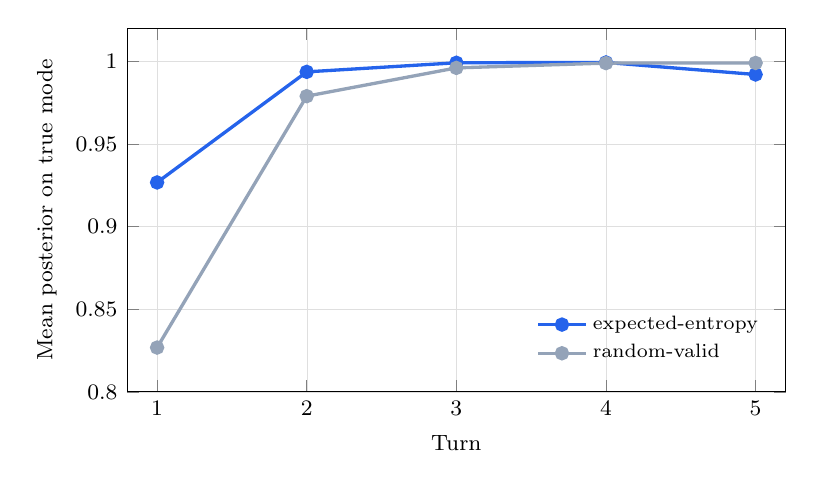
\begin{tikzpicture}
\begin{axis}[
  width=0.82\linewidth, height=6.2cm,
  xlabel={Turn},
  ylabel={Mean posterior on true mode},
  xmin=0.8, xmax=5.2,
  ymin=0.8, ymax=1.02,
  xtick={1,2,3,4,5},
  ytick={0.8,0.85,0.9,0.95,1.0},
  grid=both,
  major grid style={line width=.1pt,draw=gray!25},
  minor grid style={line width=.1pt,draw=gray!10},
  legend style={
    at={(0.98,0.05)}, anchor=south east,
    font=\scriptsize, cells={anchor=west},
    draw=none, fill=none,
  },
  tick label style={font=\footnotesize},
  label style={font=\footnotesize},
  every axis plot/.append style={line width=1.2pt, mark=*, mark size=2pt},
]
\addplot[color=stratEntropy] coordinates {
  (1, 0.9267) (2, 0.9936) (3, 0.9991) (4, 0.9993) (5, 0.9920)
};
\addplot[color=stratRandom] coordinates {
  (1, 0.8268) (2, 0.9789) (3, 0.9960) (4, 0.9989) (5, 0.9990)
};
\legend{expected-entropy, random-valid}
\end{axis}
\end{tikzpicture}
\caption{Unknown-mode posterior concentration. The entropy policy
exceeds $0.99$ confidence on the true game mode within two guesses,
while \texttt{random-valid} requires three to four. Other reasoning
policies track entropy's curve closely; the shape is governed by
the Bayes update, not the guess-selection rule.}
\label{fig:posterior}
\end{figure}

The implication for strategy design is that the mode-aware policy
\texttt{posterior-expectimax} does not actually outperform the
mode-agnostic \texttt{expected-entropy} baseline in Unknown mode.
The best Unknown-mode average is \texttt{expected-entropy} at
$4.232$ guesses; \texttt{posterior-expectimax} trails at $4.248$.
Once $q$ is close to $0$ or $1$ --- which happens within two turns
--- the blended score has already collapsed to one of its
endpoints (the Standard squared-count argmin at $q=1$, the
evil-bucket minimizer at $q=0$), so mode-aware blending only
matters during the brief window before the posterior commits.

This is a clean negative engineering result. The strategy was
designed by literally reading recurrence~(\ref{eq:VU}) and replacing
each branch with its one-ply proxy --- a textbook construction. The
reason it underperforms is mechanistic, not a bug: the Bayesian
posterior on game type concentrates fast enough that the blend
never gets a chance to do work. A different game where the
posterior decayed more slowly (longer answers, noisier feedback,
more candidate modes) would change the verdict; on this corpus
it does not.

%====================================================================
\section*{Discussion}
%====================================================================

Several findings from the benchmark were unexpected to me.

\textbf{One-step policies are nearly optimal.} I initially expected a
larger gap between greedy heuristics and the true optimum. In this
problem, however, a strategy that picks the single most informative
next guess averages only $1.3\%$ more guesses than the exact DP.
Lookahead is not useless, but the marginal benefit is modest.

\textbf{Average and worst-case metrics disagree.} Among the top
strategies, those that minimize expected guesses do not minimize the
worst case, and vice versa. Which metric to prioritize depends on the
application: minimizing the average is appropriate when many games
are played, while minimizing the worst case is appropriate when a
single-game guarantee is required.

\textbf{Adversarial worst case is easier than Standard worst case.}
In Evil mode the exact optimum is $D(A) = 4$ guesses. In Standard
mode the worst-case optimum is $W(A) = 5$: under optimal play, the
hardest fixed Wordle answer still requires $5$ guesses. The implication
is that the deterministic evil adversary is actually a weaker opponent
than the unluckiest possible fixed answer. Evil mode is only harder
than Standard mode in expectation (Standard averages $3.421$).

\textbf{Limitations and future work.} The main limitation of the
benchmark is that I could not implement an exact Standard-mode DP in
pure Python within a reasonable time budget. A natural next step
would be to vectorize the partition scoring using NumPy, which should
give a 5--10$\times$ speedup and might make the full DP feasible
overnight. A more ambitious next step would be to port the inner loop
to a compiled language.

%====================================================================
\section*{Conclusion}
%====================================================================

I constructed a benchmark harness for Wordle that evaluates six
strategies across three game variants and compares their results to
the published optima. The central finding is that simple one-step
heuristics perform remarkably well: \texttt{expected-entropy}
achieves an average of $3.465$ guesses in Standard mode, within
$0.04$ guesses of the optimum of \citet{bertsimas2022wordle}, and
\texttt{posterior-expectimax} attains the optimal Standard-mode
worst case of $5$ guesses reported by \citet{selby2022wordle}.

A second, perhaps more surprising finding concerns Unknown mode. I
expected the mode-aware blend (\texttt{posterior-expectimax}) to
beat the mode-agnostic \texttt{expected-entropy}. It does not: the
Bayesian posterior over game type concentrates above $0.99$ within
two turns, so mode-aware blending only has a brief window in which
to matter, and empirically that window is too small to move the
average. The best Unknown-mode policy on this corpus is
mode-agnostic --- a clean negative result for the engineering
hypothesis that motivated the blend in the first place.

Evil mode is the one variant where I was able to solve the recurrence
exactly in pure Python, because the adversary's deterministic
tie-breaking rule collapses the reachable state space to a few
thousand nodes. My solver recovers the published bound $D(A) = 4$
with opening guess \texttt{RAISE}. The one-guess gap between the DP
and every greedy heuristic should not be read as a general statement
about the power of dynamic programming; it is a consequence of
determinism-induced tractability in this one mode.

Compared to popular Wordle advice, these results suggest that the
commonly recommended heuristics (entropy maximization and minimax
splitting) are close enough to optimal that the residual gap is not
meaningfully exploitable by a human player. The cost of greediness is
real but small.

Finally, the benchmark's response to modeling changes is itself
informative. The information-theoretic lower bound on expected guesses
grows only as $\log_2 N$, so expected depth is relatively insensitive
to the size of the answer list. Conversely, if the evil adversary were
redefined to prefer the smallest consistent bucket, Evil mode would
collapse toward Standard mode and $D(A)$ would drop sharply. Both
perturbations are a single configuration change away in the engine,
which was one of the original motivations for developing WordleGym as
a reusable benchmark rather than a one-off analysis script.

%====================================================================

\renewcommand{\refname}{References}

\begin{thebibliography}{9}
\small
\raggedright

\bibitem[Bertsimas \& Paskov(2025)]{bertsimas2022wordle}
Bertsimas, D., \& Paskov, A.~(2025).
\newblock An exact solution to Wordle.
\newblock \emph{Operations Research}, 73(3), 1384--1394.
\newblock \url{https://doi.org/10.1287/opre.2022.0434}.
\newblock Originally circulated in 2022 as the preprint
``An Exact and Interpretable Solution to Wordle''
(\url{https://auction-upload-files.s3.amazonaws.com/Wordle_Paper_Final.pdf});
accessible summary at
\url{https://mitsloan.mit.edu/ideas-made-to-matter/how-algorithm-solves-wordle}.

\bibitem[Selby(2022)]{selby2022wordle}
Selby, A.~(2022).
\newblock The best strategies for Wordle.
\newblock \emph{sonorouschocolate.com}. Available at
\url{https://sonorouschocolate.com/notes/index.php?title=The_best_strategies_for_Wordle}.

\bibitem[Sanderson(2022)]{sanderson2022wordle}
Sanderson, G.~(2022).
\newblock Solving Wordle using information theory.
\newblock \emph{3Blue1Brown} (YouTube).
\newblock \url{https://www.youtube.com/watch?v=v68zYyaEmEA}.
\newblock Popularization of the Shannon-entropy heuristic that
underlies the \texttt{expected-entropy} strategy.

\bibitem[Shannon(1948)]{shannon1948}
Shannon, C.~E.~(1948).
\newblock A mathematical theory of communication.
\newblock \emph{The Bell System Technical Journal}, 27(3), 379--423.

\bibitem[Wardle(2022)]{wardle2022}
Wardle, J.~(2022).
\newblock Wordle [game].
\newblock \emph{The New York Times}. Canonical answer and allowed-guess lists
at \url{https://www.nytimes.com/games/wordle}.

\end{thebibliography}

\end{document}
